\chapter{Janus}
In this chapter, we will illustrate how our tool \LTLfToDFA presented in Chapter \ref{ch:ltlf2dfa} can be efficiently employed in the field of Business Process Management, with particular attention to Process Mining. First of all, we will formally describe the theoretical framework of declarative process mining, introducing a new theorem that generalizes the concept of separated formulas only for \declare constraints. Then, in this context, we will thoroughly describe the implementation of the Janus algorithm \citep{cecconi2018interestingness}, employing our tool \LTLfToDFA, for computing the interestingness degree of traces in real event logs. Finally, we will provide such a computation for a real log as an example. 
\section{Declarative Process Mining}
In this section, we will present the theoretical framework of Business Process Management focusing our attention to declarative process mining. We will extend what described in Chapter \ref{ch:theory} providing all additional concepts, definitions and theorems necessary to clearly understand the context.

Business Process Management (BPM) deals with discovering, modeling, analyzing and managing business processes in order to measure their productivity and to improve their performance. These tasks are carried out thanks to logging facilities that, nowadays, all BPM systems have. The extraction and the validation of temporal constraints from event logs (i.e. multi-sets of finite traces) are techniques consisting declarative process mining \citep{montali2010declarative}. Temporal constraints are expressed using \LTLf and/or \PLTL and refers to activities present in traces. In the following, we will formally introduce what event logs and \declare \citep{pesic2008constraint} are. Another important aspect to notice is that these constraints are meant to be checked upon the activation satisfying specific conditions. For these reasons, they are referred as \emph{reactive constraints}.
\paragraph{Event Logs}
The event log is a collection of meaningful data that is the entry point for the consequent process mining. Formally, we consider this meaningful data expressed as a multiple traces containing a sequence of events belonging to the alphabet of symbols $\Sigma$. A single trace can be represented as $t = \tup{e_1,e_2,\dots,e_n}$ where $e_i$ is the event occurring at instant $i$ and $n \in \mathbb{N}$ is the length of the trace $t$.  Now, we can give the following definition:
\begin{definition}
An event log $\L$ is defined as $\L = \{t_1,\dots,t_m\} \in \mathbb{M} (\Sigma^*)$ is a multi-set of traces $t_j$ with $1 \le j \le m$, where $m \in \mathbb{N}$.
\end{definition}
To better indicate the \textit{multiplicity} of traces in $\L$, we can denote it as a superscript compacting the notation. For example, $t_{2}^{10}$ stands for trace $t_2$ occurs $10$ times in $\L$.
\begin{example}\label{ex:traces}
$\L = \{t_{1}^{25},t_{2}^{10},t_{3}^{15},t_{4}^{20},t_{5}^{5},t_{6}^{10}\}$ is an event log of $85$ traces, defined over the alphabet $\Sigma = \{a,b,c,\dots, i \} $. In $ \L $ we have the following traces:
\begin{align*}
t_1 &= \tup{d,f,a,f,c,a,f,b,a,f}\\
t_2 &= \tup{f,e,d,c,b,a,g,h,i}\\
t_3 &= \tup{a,d,a,a,a,a,a,a,a,a,a,a,a,a,a,a,a,a,a,a,a,c}\\
t_4 &= \tup{d,b,a,b}\\
t_5 &= \tup{a,d,a,c,a}\\
t_6 &= \tup{b,c,d,e}
\end{align*}
\end{example}
Furthermore, the event $e_i$ occurring at instant $i$ is denoted by $t(i)$, whereas the segment of $t$ (i.e. the sub-trace) ranging from instant $i$ to instant $j$, where $1 \le i \le j \le n$ is denoted by $t_{[i:j]}$.

Apart from the formal model of event logs, we have real-world event logs that are logs with real data coming from different kind of data sources (e.g. databases, transaction logs, audit log, etc.). All available tools are evaluated against real-world logs. In practice, as we will see in the Section \ref{sec:janus-implementation}, the main way of representing real logs is the eXtensible Event Stream (XES) Standard\footnote{http://www.xes-standard.org}, which is based on the well known XML.
\paragraph{\declare}
\declare is a language concerning declarative process modeling \citep{pesic2008constraint} and consisting of standard templates based on \citep{dwyer1999patterns} that was introduced to simplify the complexity of constraints semantics. Indeed, \declare constraints are expressed in \LTLf, but we will extend \LTLf with Past temporal operators (\LTLp) for capturing also past modalities. In Table \ref{tab:declare-constraints}, we can see what are the corresponding \LTLf or \LTLp formulas for the most important \declare constraints.

\begin{table}[htbp]
\centering
\captionof{table}{The most important \declare constraints expressed as \LTLp formulas and \emph{reactive constraints}.}
\label{tab:declare-constraints}
\begin{tabular}{ l  c  l }
\hline
\textbf{\declare constraint} & \textbf{\LTLf expression} & \textbf{\rcon}\\
\hline
\textsc{Participation}(a) & $\Diamond a$ & $t_{start} \mapsto \Diamond a$\\
\textsc{Init}(a) & $a$ & $t_{start} \mapsto a$\\
\textsc{End}(a) & $\Box \Diamond a$ & $t_{end} \mapsto a$\\
\hline
\textsc{RespondedExistence}(a,b) & $\Diamond a \Rightarrow \Diamond b$ & $a \mapsto (\Diamond b \lOR \Once b)$\\
\textsc{Response}(a,b) & $\Box(a\Rightarrow\Diamond b)$ & $a \mapsto \Diamond b$\\
\textsc{AlternateResponse}(a,b) & $\Box(a\Rightarrow\Diamond b) \lAND \Box(a\Rightarrow \Next(\lnot a \Wnext b))$ & $a \mapsto \Next( \lnot a \lUntil b)$\\
\textsc{ChainResponse}(a,b) & $\Box(a\Rightarrow\Diamond b) \lAND \Box(a\Rightarrow \Next b)$ & $a \mapsto \Next b$\\
\textsc{Precedence}(a,b) & $\lnot b \Wnext a$ & $b \mapsto \Once a$\\
\textsc{AlternatePrecedence}(a,b) & $(\lnot b \Wnext a) \lAND \Box(a\Rightarrow \Next(\lnot b \Wnext a))$ & $b \mapsto \Yesterday(\lnot b \Since a)$\\
\textsc{ChainPrecedence}(a,b) & $(\lnot b \Wnext a) \lAND \Box(\Next b\Rightarrow a)$ & $b \mapsto \Yesterday a$\\
\hline
\end{tabular}
\end{table}

%\begin{figure}[h]
%\centering
%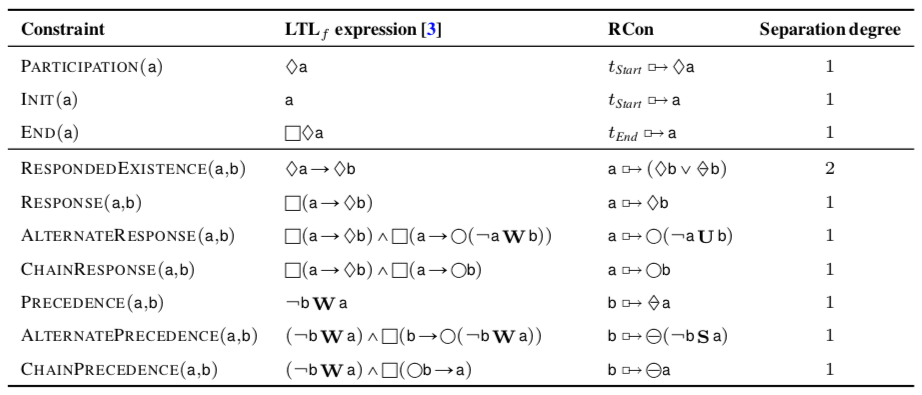
\includegraphics[width=\textwidth]{images/declare-constraints}
%\caption{The most important \declare constraints expressed as \LTLf formulas and \emph{reactive constraints}.}
%\label{fig:declare-constraints}
%\end{figure}
Parameters in a template define tasks and they occurs as events in traces. In Example \ref{ex:declare-examples} we provide a glimpse of \declare patterns.
\begin{example}\label{ex:declare-examples}
Interesting \declare templates \citep{maggi2013knowledge}
\begin{itemize}
\item \textsc{Precedence}(a,b) means \emph{if b occurs then a occurs before b}.
\item \textsc{Responce}(a,b) means \emph{if a occurs then eventually b occurs after a}.
\item \textsc{ChainPrecedence}(a,b) means \emph{the occurrence of b imposes a to occur immediately before}.
\item \textsc{AlternateResponce}(a,b) means \emph{if a occurs then eventually
b occurs after a without other occurrences of a in between}.
\end{itemize}
\end{example}
In addition, one can create his own 	\declare patterns tailored for his purposes. In this way, the \declare standard template can be customized.

A given \declare constraint is verified over traces and those traces \emph{satisfy} it if they do not \emph{violate} it. Here, it is important to notice that these constraints are prone to the principle of \textit{ex falso quod libet}, namely they can be satisfied even without being activated. This represents a big issue for process mining because mining techniques might misunderstand the actual behavior of a process. The solution to this problem is to compute whether a constraint is satisfied or not only upon activation. However, we will see later how to overcome this problem in the Section \ref{sec:janus}.

Now, we give some definitions:
\begin{definition}\citep{gabbay1989declarative}\label{def:pure-temp-formula}
Given an \LTLp formula $\varphi$, we call it \emph{pure past} formula ($\varphi^\blacktriangleleft$) if it consists of only past operators; \emph{pure present} formula ($\varphi^\blacktriangledown$) if it has not any temporal operators; \emph{pure future} formula ($\varphi^\blacktriangleright$) if it consists of only future operators.
\end{definition}
\begin{example}\label{ex:pure-formulas-examples}
Pure formulas:
\begin{itemize}
\item $\boxminus(a \Rightarrow \Once b)$ is a \textbf{pure past} formula;
\item $a \Rightarrow (b \lAND c)$ is a \textbf{pure present} formula
\item $\Box(a \Rightarrow \Next b)$ is a \textbf{pure future} formula
\end{itemize}
\end{example}
The separation of an \LTLp formula to pure past/present/future formulas allows to conduct the analysis on sub-traces (i.e. one referring to the past and the other referring to the future) upon the activation. This is also known as bi-directional on-line analysis. To this extent, we rely on the Separation Theorem stated as follows:
\begin{theorem}\citep{gabbay1989declarative}\label{th:separation-theorem}
Any propositional temporal formula $\varphi$ can be rewritten as a boolean combination of pure temporal formulas.
\end{theorem}
Therefore, following Theorem \ref{th:separation-theorem}, we can give the Definition of \textit{separated formula} as follows:
\begin{definition}\citep{cecconi2018interestingness}\label{def:separated-formula}
Let  $\varphi$ an \LTLp formula over $\Sigma$. A temporal separation is a function $\S: \textsc{ltl}p_f  \rightarrow 2^{\textsc{ltl}p_f \times \textsc{ltl}p_f 	\times \textsc{ltl}p_f}$ such that: $\S(\varphi) = \{(\varphi^{\blacktriangleleft},\varphi^{\blacktriangledown},\varphi^{\blacktriangleright})_1,\dots,\\(\varphi^{\blacktriangleleft},\varphi^{\blacktriangledown},\varphi^{\blacktriangleright})_m\}$ such that:
\begin{equation}\label{eq:separated-formulas}
\varphi \equiv \bigvee^{m}_{j=1} (\varphi^{\blacktriangleleft} \lAND \varphi^{\blacktriangledown} \lAND \varphi^{\blacktriangleright})_j
\end{equation}
where $\varphi^\blacktriangleleft$, $\varphi^\blacktriangledown$ and $\varphi^\blacktriangleright$ are pure formulas over $\Sigma$ as in Definition \ref{def:pure-temp-formula}.
\end{definition}
Notice that Equation \ref{eq:separated-formulas} is a disjunction of conjunction. Moreover, each triple consisting the image function of $\S(\varphi)$ is generally called \emph{separated formula}. In the following, we give an example of separated formula.
\begin{example}\label{ex:separated-formulas}
The separated formulas for $(\Yesterday a \lOR \Diamond b$):
\begin{align*}
(\Yesterday a \lAND True \lAND True)\bigvee(True \lAND True \lAND \Diamond b)
\end{align*}
\end{example}
PUT HERE THE NEW GENERALIZATION OF THE THEOREM

Since the Janus algorithm relies on the construction of the automata for separated \LTLp formulas, we will refer to notions explained previously in Section \ref{sec:formula-to-automa}. The crucial point is that given a separated \LTLp formula $\varphi$ we can build a minimum \DFA that \emph{accepts} all and only the traces satisfying formula $\varphi$.

In the following sections, we will describe in details the Janus approach giving fundamentals definitions and theorems. Then, we will illustrate the algorithm and its practical implementation.
\section{Janus}\label{sec:janus}
Declarative process modeling defines a list of \declare constraints to be satisfied during the execution of the process model. These constraints are of a reactive nature in the sense that the occurrence of some task bounds the occurrence of other activities. As anticipated in the previous Section, this kind of behavior might lead to the principle of \textit{ex falso quod libet}, namely a constraint can be satisfied even though it is never activated. Here, the Janus approach \citep{cecconi2018interestingness} solves this problem allowing the user to indicate the activation condition for the constraint directly in the constraint formula. In this way, constraints are activated only if the activation condition holds. Therefore, we can refer to these constraints as \textit{reactive constraints} (\rcon).
\begin{definition}\citep{cecconi2018interestingness}\label{def:rcon}
Given an alphabet $\Sigma$, let $\alpha \in \Sigma$ be an \emph{activation} and $\varphi$ be an \LTLp formula over $\Sigma$. A Reactive Constraint (\rcon) $\Psi$ is a pair $(\alpha, \varphi)$, denoted as $\Psi \doteq \alpha  \mapsto \varphi$. We represent all the set of \rcon s over $\Sigma$ as $\mathcal{R}$.
\end{definition}
Hereafter, we will assume traces, automata, \LTLp formulas and \rcon s to be defined over the same alphabet $\Sigma$. In addition, in Table \ref{tab:declare-constraints}, we can see that \declare constraints can be converted in \rcon s. In Definition \ref{def:rcon}, we have seen that $\alpha$ in an \rcon\xspace is called the \emph{activation}. Indeed, it actually \emph{activates} the corresponding constraint. As in \citep{cecconi2018interestingness}, we give the following definitions that are the core concepts upon which the Janus algorithm is built.
\begin{definition}\citep{cecconi2018interestingness}\label{def:activator}
Given a finite trace $t \in \Sigma$ of length $n$, and an instant $i$, with $1 \le i \le n$, an \rcon\xspace $\Psi \doteq \alpha  \mapsto \varphi$ is activated at $i$ if $t,i \models \alpha$. Thus, the event $t(i)$ is called the \emph{activator} of $\Psi$. A trace in which at least an activator of $\Psi$ exists, is \emph{triggering} for $\Psi$.
\end{definition}

\begin{definition}\citep{cecconi2018interestingness}\label{def:interesting-fulfilment}
Given a finite trace $t \in \Sigma$ of length $n$, an instant $i$, with $1 \le i \le n$, an \rcon\xspace $\Psi \doteq \alpha  \mapsto \varphi$, $\Psi$ is \emph{interesting fulfilled} at $i$ if $t,i \models \alpha$ and $t,i \models \varphi$. The \rcon\xspace is \emph{violated} at instant $i$ if $t,i \models \alpha$ and $t,i \not\models \varphi$. Otherwise, the \rcon\xspace is unaffected.
\end{definition}

Definition \ref{def:interesting-fulfilment} is called \textit{interesting fulfilment}, since it formally solves the problem of constraint satisfaction without activation by identifying only those events where the activation condition holds and the \rcon\xspace is fulfilled. Therefore, every time an event is the activator of an \rcon, the \rcon\xspace is checked for fulfilment.
After these two definitions we have to define also an empirical method to compute the \textit{interesting fulfilment} of an \rcon\xspace for an event log.

\begin{definition}\citep{cecconi2018interestingness}\label{def:interestingness-degree}
Given a finite trace $t \in \Sigma$ of length $n$ and an \rcon\xspace $\Psi \doteq \alpha  \mapsto \varphi$, we define the \emph{interestingness degree} function $\zeta: \mathcal{R} \times \Sigma^* \rightarrow [0,1] \subseteq \mathbb{R}$ as follows:
\[   
\zeta(\Psi,t) = 
     \begin{cases}
       \dfrac{\lvert \{ i: t,i \models \alpha \text{ and } t,i \models \varphi\} \rvert}{\lvert \{ i: t,i \models \alpha\} \rvert}, &\quad\text{if } \lvert \{ i: t,i \models \alpha\} \rvert \neq 0 ;\\
       0, &\quad\text{otherwise} \\
     \end{cases}
\]
\end{definition}
Intuitively, the $\zeta(\Psi, t)$ function measures how many times the \rcon\xspace $\Psi$ is interesting fulfilled with respect to the total number of activations within the trace $t$. In Section \ref{sec:janus-implementation}, we will see the implementation of the Janus algorithm for computing the \emph{interestingness degree} of traces in real-world event logs.
Now, we give an example to better capture the concepts just defined.

\begin{example}\label{ex:janus-interest}
Let us consider the \rcon\xspace $\Psi = b \mapsto \Once a$ and traces in the Example \ref{ex:traces}, we have the following:
\begin{itemize}
\item $\Psi$ is activated in trace $t_1$ by $t_1(8)$, in $t_2$ by $t_2(5)$, in $t_4$ by $t_4(2)$ and $t_4(4)$ and in $t_6$ by $t_6(1)$. Hence, $t_1$, $t_2$, $t_4$ and $t_6$ are \textit{triggering} for $\Psi$, while $\Psi$ is not activated in $t_3$ and $t_5$.
\item $\Psi$ is \textit{interestingly fulfilled} by $t_1(8)$ in $t_1$, by only $t_4(4)$ in $t_4$. Moreover, $\Psi$ is \textit{violated} by $t_2(5)$ in $t_2$, by $t_4(2)$ in $t_4$ and by $t_6(1)$ in $t_6$. Finally, it is \textit{unaffected} both in $t_3$ and $t_5$. 
\item The \textit{interestingness degree} of $\Psi$ in $t_1$ is $\zeta(\Psi, t_1) = 1$, since it is activated and fulfilled only once. Then, the \textit{interestingness degree} of $\Psi$ in $t_4$ is $\zeta(\Psi, t_4) = 0.5$ because it is activated twice, but fulfilled only once. Finally, in all the other traces $t_2$, $t_3$, $t_5$ and $t_6$ is $\zeta(\Psi, t) = 0$.
\end{itemize}
\end{example}
As we have just seen, the fulfilment of an \rcon\xspace, in a trace, relies on the verification of the corresponding \LTLp formula over such a trace at the instant of activation. This process of verification of a formula $\varphi$ on a trace can be achieved by constructing the related \DFA $\automaton_{\varphi}$ and checking whether such trace is accepted by $\automaton_{\varphi}$ or not. To this extent, in the following, we have to give some other definitions and theorems.

First of all, since an \LTLp formula could have both past and future temporal operators, in order to build its corresponding \DFA we exploit the Theorem \ref{th:separation-theorem} by first splitting the \LTLp formula into its separated formulas and, then, constructing the corresponding \DFAs of that separated formulas. However, we need to know how to evaluate the separated formulas over a trace. We can now give the following Lemma and Theorem:

\begin{lemma}\citep{cecconi2018interestingness}\label{lem:subtrace-eval}
Given a pure past formula $\varphi^\blacktriangleleft$, a pure present formula $\varphi^\blacktriangledown$, a pure future formula $\varphi^\blacktriangleright$, a finite trace $t \in \Sigma^*$ of length $n$ and an instant $i$, with $1 \le i \le n$, the following is holds true:
\begin{itemize}
\item $t,i \models \varphi^\blacktriangleleft \equiv t_{[1,i]}, i \models \varphi^\blacktriangleleft$
\item $t,i \models \varphi^\blacktriangledown \equiv t_{[i,i]}, i \models \varphi^\blacktriangledown$
\item $t,i \models \varphi^\blacktriangleright \equiv t_{[i,n]}, i \models \varphi^\blacktriangleright$
\end{itemize}
\end{lemma}
The Lemma follows from the definition of the \LTLp semantics. It is trivial to see that having, at instant $i$, a pure past formula, its semantics only cares about events preceding $i$, whereas a pure future formula cares only about events following the instant $i$.
\begin{theorem}\citep{cecconi2018interestingness}\label{th:sepformulas-eval}
Given an \LTLp formula $\varphi$, a finite trace $t \in \Sigma^*$ of length $n$ and an instant $i$, with $1 \le i \le n$, we have that $t,i \models \varphi \tiff t_{[1,i]}, i \models \varphi^\blacktriangleleft, t_{[i,i]}, i \models \varphi^\blacktriangledown$ and $t_{[i,n]}, i \models \varphi^\blacktriangleright$ for \emph{at least} a $(\varphi^{\blacktriangleleft},\varphi^{\blacktriangledown},\varphi^{\blacktriangleright}) \in \S(\varphi)$.
\end{theorem}
The proof follows from Theorem \ref{th:separation-theorem} and Lemma \ref{lem:subtrace-eval}.

\begin{example}\label{ex:subeval-formula}
Let us consider the \rcon\xspace $\Psi = a \mapsto (\Yesterday b \lOR \Diamond c)$ with $\varphi = (\Yesterday b \lOR \Diamond c)$, its separated formulas $\S(\varphi) = \{(\Yesterday b , True, True),(True, True, \Diamond c)\}$ and trace $t_1 = \tup{d,f,a,f,c,a,f,b,a,f}$ taken from Example \ref{ex:traces}.
\begin{itemize}
\item $t_1,3 \models \varphi$ if, apart from the $True$ formulas that are satisfied, one of the following holds $\true$:
\begin{enumerate}
\item $\tup{d,f,a},3 \models \Yesterday b$
\item $\tup{a,f,c,a,f,b,a,f},3 \models \Diamond c$
\end{enumerate}
since the latter holds $\true$, $\varphi$ is satisfied by $t_1(3)$.

\item $t_1,6 \models \varphi$ if, apart from the $True$ formulas that are satisfied, one of the following holds $\true$:
\begin{enumerate}
\item $\tup{d,f,a,f,c,a},6 \models \Yesterday b$
\item $\tup{a,f,b,a,f},6 \models \Diamond c$
\end{enumerate}
since both are not satisfied, we can conclude that $\varphi$ is not satisfied by $t_1(6)$.

\item $t_1,9 \models \varphi$ if, apart from the $True$ formulas that are satisfied, one of the following holds $\true$:
\begin{enumerate}
\item $\tup{d,f,a,f,c,a,f,b,a},9 \models \Yesterday b$
\item $\tup{a,f},9 \models \Diamond c$
\end{enumerate}
since the former holds $\true$, $\varphi$ is satisfied by $t_1(9)$.
\end{itemize}
\end{example}
At this point, we can start talking about separated formulas verification on a trace using their corresponding \DFAs. 

\begin{definition}\citep{cecconi2018interestingness}\label{def:automaton-eval}
Given a \LTLp formula $\varphi$, we define as \emph{separated automata set} (sep.aut.set) $\automaton^{\blacktriangleleft \blacktriangledown \blacktriangleright} \in 2^{\automaton \x \automaton \x \automaton}$ the set of triples $\automaton^{\blacktriangleleft \blacktriangledown \blacktriangleright} = (\automaton^{\blacktriangleleft}, \automaton^{\blacktriangledown}, \automaton^{\blacktriangleright}) \in \automaton \x \automaton \x \automaton$ such that $\automaton^{\blacktriangleleft} \doteq \automaton_{\varphi^\blacktriangleleft}$, $\automaton^{\blacktriangledown} \doteq \automaton_{\varphi^\blacktriangledown}$ and $\automaton^{\blacktriangleright} \doteq \automaton_{\varphi^\blacktriangleright}$ for every $(\varphi^{\blacktriangleleft},\varphi^{\blacktriangledown},\varphi^{\blacktriangleright}) \in \S(\varphi)$.
\end{definition}
As in Example \ref{ex:separated-formulas}, here we give its automata version.
\begin{example}\label{ex:automata-sep-formulas}
The sep.aut.set for $(\Yesterday a \lOR \Diamond b$) is:
\begin{align*}
\automaton^{\blacktriangleleft \blacktriangledown \blacktriangleright} = \{(\automaton_{\Yesterday a}, \automaton_{True}, \automaton_{True}), (\automaton_{True}, \automaton_{True}, \automaton_{\Diamond b})\}
\end{align*}
\end{example}
Similarly to what we have seen before with Theorem \ref{th:sepformulas-eval}, we can state the following:

\begin{theorem}\citep{cecconi2018interestingness}\label{th:sepformulas-eval}
Given an \LTLp formula $\varphi$, its sep.aut.set $\automaton^{\blacktriangleleft \blacktriangledown \blacktriangleright}$, a finite trace $t \in \Sigma^*$ of length $n$ and an instant $i$, with $1 \le i \le n$, we have that $t,i \models \varphi \tiff t_{[1,i]}, i \in \L(\automaton^\blacktriangleleft), t_{[i,i]}, i \in \L(\automaton^\blacktriangledown)$ and $t_{[i,n]}, i \in \L(\automaton^\blacktriangleright)$ for \emph{at least} a $(\automaton^{\blacktriangleleft}, \automaton^{\blacktriangledown}, \automaton^{\blacktriangleright}) \in \automaton^{\blacktriangleleft \blacktriangledown \blacktriangleright}$.
\end{theorem}

So far, we have described all theoretical results necessary for introducing and understanding how the Janus algorithm works. Now, we talk about automata generation given a pure past, pure present and a pure future formula possible thanks to our developed tool \LTLfToDFA. 

Differently from what has been done in \citep{cecconi2018interestingness} for the automata construction, in this thesis we propose a version of the Janus algorithm that works with \LTLfToDFA. Indeed, as already seen in Chapter \ref{ch:ltlf2dfa}, \LTLfToDFA is able to directly generate the minimum \DFA for a pure past formula (\PLTL) without passing through its pure future (\LTLf) reversed formula. In particular, \LTLfToDFA has been employed in the Janus algorithm for the generation of the automaton corresponding to each formula in the triple $(\varphi^{\blacktriangleleft},\varphi^{\blacktriangledown},\varphi^{\blacktriangleright})$, for every triple $(\varphi^{\blacktriangleleft},\varphi^{\blacktriangledown},\varphi^{\blacktriangleright}) \in \S(\varphi)$. In Example \ref{ex:sep-aut-set}, there are the \DFAs output from \LTLfToDFA.

\begin{example}\label{ex:sep-aut-set}
Let us consider the \rcon\xspace $\Psi = a \mapsto (\Yesterday b \lOR \Diamond c)$ and its separated formula $\S(\varphi) = \{(\Yesterday b , True, True), (True, True, \Diamond c)\}$. The corresponding sep.aut.set $\automaton^{\blacktriangleleft \blacktriangledown \blacktriangleright}$ for each $(\varphi^{\blacktriangleleft},\varphi^{\blacktriangledown},\varphi^{\blacktriangleright}) \in \S(\varphi)$ is depicted in Table \ref{tab:sep-aut-set}:
\begin{center}
\captionof{table}{Representation of the separated automata set for $\Psi = a \mapsto (\Yesterday b \lOR \Diamond c)$}
\label{tab:sep-aut-set}
\begin{tabular}{ c  c  c }
\hline
$\automaton^{\blacktriangleleft} = \automaton_{\Yesterday b}$ & $\automaton^{\blacktriangledown} = \automaton_{\true}$ & $\automaton^{\blacktriangleright} = \automaton_{\true}$\\
\hline
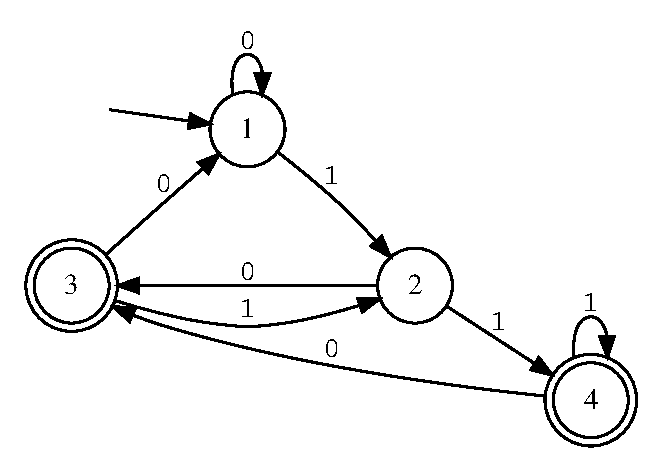
\includegraphics[width=0.3\textwidth]{images/automa3-yesterday.eps}
&
\raisebox{.7\height}{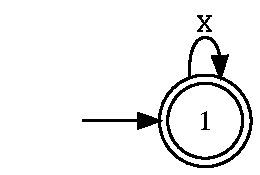
\includegraphics[width=0.1\textwidth, height=3.5em]{images/automa4-true.eps}}
&
\raisebox{.7\height}{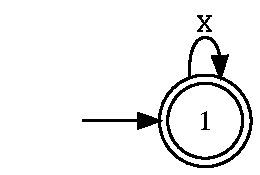
\includegraphics[width=0.1\textwidth, height=3.5em]{images/automa4-true.eps}}\\
\hline
$\automaton^{\blacktriangleleft} = \automaton_{\true}$ & $\automaton^{\blacktriangledown} = \automaton_{\true}$ & $\automaton^{\blacktriangleright} = \automaton_{\Diamond c}$\\
\hline
\raisebox{.4\height}{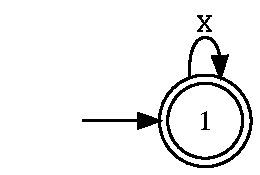
\includegraphics[width=0.1\textwidth, height=3.5em]{images/automa4-true.eps}}
&
\raisebox{.4\height}{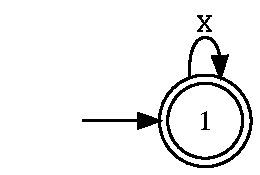
\includegraphics[width=0.1\textwidth, height=3.5em]{images/automa4-true.eps}}
&
\raisebox{.07\height}{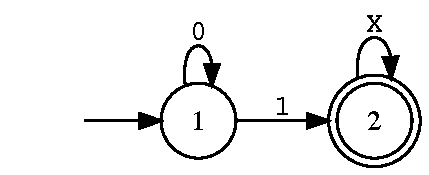
\includegraphics[width=0.3\textwidth]{images/example1-output.eps}}\\
\hline
\end{tabular}
\end{center}
\end{example}
\subsection{Algorithm}\label{sec:janus-alg}
\section{Implementation}\label{sec:janus-implementation}
In this section, we fully describe the practical implementation of the Janus algorithm given in Section \ref{sec:janus-alg}. In particular, we give some general information about its features, dependencies and usage. Then, we focus on the package explaining how is structured and commenting highlights on the code. The implementation on this thesis is called \janus, is written in Python and is a porting of the \href{https://github.com/Oneiroe/Janus}{Janus} proof-of-concept software project written in Java.

To begin with, the main goal of \janus, as stated at the beginning, is to compute the \textit{interestingness degree} of traces on event log.  As a consequence, it also provides I/O facilities for three different event log formats, namely simple \textit{.txt} files, \textit{.csv} files and \textit{.xes} files for real-world event logs. Furthermore, the formula $\varphi$ in the \rcon\xspace to be satisfied by traces is manually separated following Definition \ref{def:separated-formula}.

\janus requires Python>=3.6 and has the following dependencies:
\begin{itemize}
\item \LTLfToDFA, presented in Chapter \ref{ch:ltlf2dfa}. As stated before, it has been used for the generation of \DFAs;
\item \href{https://github.com/opyenxes/OpyenXes}{OpyenXES}, an open-source complete Python library for the XES Standard published in \citep{DBLP:conf/bpm/ValdiviesoLMS18}. It has been used for dealing with XES parsing and management.
\end{itemize} 
The \janus software is an open-source project and available to download on GitHub\footnote{https://github.com/Francesco17/janus}.
\subsection{Package Structure}
The structure of the \janus package is relatively simple. It consists of the following:
\begin{itemize}
\item \texttt{janus.py}: it is the main module of the package. It contains the actual implementation of the Janus algorithm.
\item \texttt{janus/}: it is the directory containing all the necessary code to correctly implement the algorithm. It has three subfolders:
\begin{itemize}
\item  \texttt{io/}: it contains the \texttt{InputHandler.py} which is in charge of handling the event log given as input.
\item \texttt{automata/}: it consists of the \texttt{automa.py} file, the \texttt{parserAutoma.py} file and the \texttt{sepautset.py} file. In this folder, we find all the code for dealing with automata.
\item \texttt{formulas/}: it comprises the \texttt{formula.py} file and the \texttt{separatedFormula.py}. These files defines the logic for \LTLp formulas and \rcon s.
\end{itemize}
\item \texttt{files/}: this folder is the place where there are event logs. From this folder, a specific event log is parsed.
\end{itemize}
\subsection{I/O}
The \texttt{InputHandler.py} file, included in the \texttt{io/} folder, has been developed separately from the main module since we wanted to use our algorithm regardless of the input file format. In particular, thanks to the relative \texttt{InputHandler} class (Listing \ref{code:janus-input}), the tool can import a log from a simple text file, from a csv and, finally, from a XES file. Hence, the \janus tool can be used not only with the XES format, but also with other more manageable file formats.
\begin{lstlisting}[language=Python, style=Python, escapechar = £, label={code:janus-input}, caption={The \texttt{InputHandler.py} module}]
import csv
from opyenxes.data_in.XUniversalParser import XUniversalParser
from opyenxes.classification.XEventAttributeClassifier import \
XEventAttributeClassifier

class InputHandler:

    def __init__(self, input_path):
        self.input_path = input_path
        self._event_log = None
        self.load()

    @property
    def event_log(self):
        return self._event_log

    def load_txt(self):
        try:
            with open(self.input_path, 'r') as f:
                self._event_log = set(tuple(i) for i in \
                [f.read().splitlines()])
                f.close()
        except:
            raise IOError('[ERROR]: Unable to import text file')

    def load_csv(self):
        self._event_log = []
        try:
            with open(self.input_path, newline='', encoding='utf-8-sig') \
            as f:
                reader = csv.reader(f)
                for row in reader:
                    self._event_log.append(row[0])
        except:
            raise IOError('[ERROR]: Unable to import csv file')

    def load_xes(self):£\label{line:load-xes}£
        try:
            with open(self.input_path) as log_file:
                log = XUniversalParser().parse(log_file)[0]

            # get classifiers
            classifiers = []
            for cl in log.get_classifiers():
                classifiers.append(str(cl))

            classifier = XEventAttributeClassifier("activity", \
            [classifiers[0]])
            log_list = list(map(lambda trace: \
            (map(classifier.get_class_identity, trace)), log))

            self._event_log = set(tuple(trace) for trace in log_list)

        except:
            raise IOError('[ERROR]: Unable to import xes file')

    def load(self):
        if self.input_path.endswith('.txt'):
            self.load_txt()
        elif self.input_path.endswith('.csv'):
            self.load_csv()
        elif self.input_path.endswith('.xes'):
            self.load_xes()
        else:
            raise ValueError('[ERROR]: File extension not recognized')
\end{lstlisting}
From Listing \ref{code:janus-input}, we can see that the \texttt{InputHandler} class has a main method called \texttt{load} that depending on the format of the file given as input calls the corresponding method specific for that format. If the format is not among \textit{.txt}, \textit{.csv} and \textit{.xes}, it raises an error.
Consequently, every specific method parses the event log. In particular, at line \ref{line:load-xes}, the \texttt{load\_xes} method takes advantage of the OpyenXES library APIs using its parser and classifier. In Section \ref{sec:janus-main}, we will look at how an \texttt{InputHandler} object can be instantiated.
\subsection{Automata}
In the \texttt{automata/} folder there are files devoted to handle and manage automata. Firstly, the \texttt{parserAutoma.py} module is a collection of functions used for parsing the \textit{.dot} file and instantiating the data structure representing the automaton. In Listing \ref{code:janus-parser-automa} is shown that collection of functions.
\begin{lstlisting}[language=Python, style=Python, escapechar = £, label={code:janus-parser-automa}, caption={The \texttt{parserAutoma.py} module}]
import pydot
from janus.automata.automa import Automa

def get_file(path):
    try:
        with open(path, 'r') as file:
            lines = file.readlines()
            file.close()
        return lines
    except IOError:
        print('[ERROR]: Not able to open the file from {}'.format(path))

def get_graph_from_dot(path):
    try:
        dot_graph = pydot.graph_from_dot_file(path)
        return dot_graph[0]
    except IOError:
        print('[ERROR]: Not able to import the dot file')

def get_final_label(label):

    s1 = label.replace(" ", "")
    s2 = s1.replace('"','')

    if s2 == '':
        return ['X']
    elif len(s2) < 2:
        return [s2]
    else:
        s3 = s2.replace(",","")
        s4 = s3.split('\\n')

        leng_elem = len(s4[0])
        temp = ''
        inter_label = []
        for i in range(leng_elem):
            for elem in s4:
                temp += elem[i]
            inter_label.append(temp)
            temp = ''

        return inter_label

def parse_dot(path, symbols):£\label{line:parse-dot}£

    graph = get_graph_from_dot(path)

    nodes = []
    for node in graph.get_nodes():
        if node.get_name().isdigit():
            nodes.append(node.get_name())
        else: continue

    states = set(nodes)
    initial_state = sorted(nodes, key=int)[0]

    lines = get_file(path)
    accepting_states = set() # all accepting states of the automaton
    for line in lines[7:]:
        if line.strip() != 'node [shape=circle];':
            temp = line.replace(";\n", "")
            accepting_states.add(temp.strip())
        else:
            break

    sources = []
    for elem in graph.get_edges():
        if elem.get_source().isdigit():
            sources.append(elem.get_source())
        else: continue

    i = 0
    transitions = dict()
    for source in sources:
        label = graph.get_edges()[i].get_label()
        final_label = get_final_label(label)
        destination = graph.get_edges()[i].get_destination()
        i += 1
        for lab in final_label:
            if source in transitions:
                transitions[source][lab] = destination
            else:
                transitions[source] = dict({lab: destination})

    #instantiation of automaton
    automaton = Automa(
        symbols=symbols,
        alphabet={'0', '1', 'X'},
        states=states,
        initial_state=initial_state,
        accepting_states=accepting_states,
        transitions=transitions
    )
    return automaton
\end{lstlisting}
The most important function is called \texttt{parse\_dot} (at line \ref{line:parse-dot}). It works as follows: given the path of a \textit{.dot} file (the output of \LTLfToDFA) and symbols used in the formula, it returns an instantiation of the \texttt{Automa} class retrieving all information about the \DFA, namely all its states, the initial state, accepting states and, finally, its transitions.

Afterwards, there is the \texttt{automa.py} in which the \texttt{Automa} class is implemented. This class is the data structure representing the \DFA that is output from our tool \LTLfToDFA. It follows that in the \texttt{Automa} class there are methods able to perform transitions over the \DFA, to tell whether if the automaton is in an accepting state or not and to tell whether an input symbols can be read by the automaton or not. In addition, when an object is instantiated, it is checked to be a valid \DFA. In Listing \ref{code:janus-automa} the \texttt{Automa} class implementation is shown.
\begin{lstlisting}[language=Python, style=Python, escapechar = £, label={code:janus-automa}, caption={The \texttt{automa.py} module}]
import re

class Automa:
    """
        DFA Automa:
        - symbols          => list() ;
        - alphabet         => set() ;
        - states           => set() ;
        - initial_state    => str() ;
        - accepting_states => set() ;
        - transitions      => dict(), where
        **key**: *source* in states
        **value**: {*action*: *destination*)
    """

    def __init__(self, symbols, alphabet, states, initial_state, \
    accepting_states, transitions):
        self.symbols = symbols
        self.alphabet = alphabet
        self.states = states
        self._initial_state = initial_state
        self.accepting_states = accepting_states
        self.transitions = transitions
        self._current_state = self._initial_state
        self.validate()

    def valide_transition_start_states(self):
        for state in self.states:
            if state not in self.transitions:
                raise ValueError(
                    'transition start state {} is missing'.format(
                        state))

    def validate_initial_state(self):
        if self._initial_state not in self.states:
            raise ValueError('initial state is not defined as state')

    def validate_accepting_states(self):
        if any(not s in self.states for s in self.accepting_states):
            raise ValueError('accepting states not defined as state')

    def validate_input_symbols(self):
        alphabet_pattern = self.get_alphabet_pattern()
        for state in self.states:
            for action in self.transitions[state]:
                if not re.match(alphabet_pattern, action):
                    raise ValueError('invalid transition found')

    def get_alphabet_pattern(self):
        return re.compile("(^["+''.join(self.alphabet)+"]+$)")

    def validate(self):£\label{line:dfa-validation}£
        self.validate_initial_state()
        self.validate_accepting_states()
        self.valide_transition_start_states()
        self.validate_input_symbols()
        return True

    ...

    @property
    def current_state(self):
        return self._current_state

    @property
    def initial_state(self):
        return self._initial_state

    def make_transition(self, action):£\label{line:make-trans}£
        if action in self.symbols:
            for act in self.transitions[self._current_state].keys():
                temp = dict(zip(self.symbols,[value for value in act]))
                additional = temp.copy()
                del additional[action]
                if (temp[action] == '1' or temp[action] == 'X') and \
                all(value in {'0', 'X'} for value in additional.values()):
                    self._current_state = \
                    self.transitions[self._current_state][act]
                else:
                    continue
        else:
            number_of_symbols = len(self.symbols)
            if number_of_symbols == 0: # true when there is True automa
                self._current_state = \
                self.transitions[self._current_state]['X']
            else:
                if 'X'*number_of_symbols in \
                self.transitions[self._current_state]:
                    self._current_state = \
                    self.transitions[self._current_state]\
                    ['X'*number_of_symbols]
                elif '0'*number_of_symbols in \
                self.transitions[self._current_state]:
                    self._current_state = \
                    self.transitions[self._current_state]\
                    ['0'*number_of_symbols]
                else:
                    raise ValueError('[ERROR]: could not make transition')

    def is_accepting(self):£\label{line:is-accepting}£
        if self._current_state in self.accepting_states:
            return True
        else:
            return False

    def accepts(self, input_symbol):£\label{line:accepts}£
        _current_state = self._current_state
        self._current_state = self._initial_state
        self.make_transition(input_symbol)
        if self.is_accepting():
            self._current_state = _current_state
            return True
        else:
            self._current_state = _current_state
            return False
\end{lstlisting}
Once an \texttt{Automa} object is instantiated, the method \texttt{validate} (line \ref{line:dfa-validation}) checks whether the object is a valid \DFA or not. In particular, it checks if the initial state and final states are actually states and it verifies that transitions are not made by invalid symbols.
Then, the \texttt{make\_transition} method at line \ref{line:make-trans} takes as input an action and make this action on the automaton, therefore modifying its current state. After that, the \texttt{is\_accepting} method (line \ref{line:is-accepting}) simply tells whether the current state is accepting for the automaton itself or not. Finally, there is the \texttt{accepts} method at line \ref{line:accepts}, which given an input symbol returns $\true$ if it is accepted by the \DFA.

As last module about automata, we illustrate the \texttt{sepautset.py}. It is the direct implementation of the \textit{sep.aut.set} defined in \ref{def:automaton-eval}. Indeed, this module contains the definition of the \texttt{SeparatedAutomataSet} class, namely the data structure that allow us to generate the corresponding \textit{sep.aut.set}. Hence, it takes care of generating the set of separated automata starting from a list of separated formulas. We can see its implementation in Listing \ref{code:janus-sepautset}.
\begin{lstlisting}[language=Python, style=Python, escapechar = £, label={code:janus-sepautset}, caption={The \texttt{sepautset.py} module}]
from ltlf2dfa.Translator import Translator
from ltlf2dfa.DotHandler import DotHandler
from janus.automata.parserAutoma import parse_dot
import os, re

class SeparatedAutomataSet:

    def __init__(self, separated_formulas_set):
        self.separated_formulas_set = separated_formulas_set
        self._automa_set = self.compute_automa()

    @property
    def automa_set(self):
        return self._automa_set

    def build_automaton(self, triple):£\label{line:build-dfa}£
        automata_list = []
        for formula in triple:
            symbols = re.findall('[a-z]+', str(formula))
            trans = Translator(formula)
            trans.formula_parser()
            trans.translate()
            trans.createMonafile(True)  # true for DECLARE assumptions
            trans.invoke_mona("automa.mona") # returns inter-automa.dot
            dot = DotHandler("inter-automa.dot")
            dot.modify_dot()
            dot.output_dot() # returns automa.dot
            automata_list.append(parse_dot("automa.dot", symbols))
            os.remove("automa.mona")
            os.remove("automa.dot")
            symbols = []
        return automata_list

    def compute_automa(self):
        result = set()
        for triple in self.separated_formulas_set:£\label{line:automa-set}£
            past, present, future = self.build_automaton(triple)
            result.add( (past, present, future) )
        return result
\end{lstlisting}
In this module, it has been employed the \LTLfToDFA tool. In fact, a \texttt{SeparatedAutomataSet} object receives a given set of separated formulas as input and it uses \LTLfToDFA to generate the \DFA corresponding to each formula. Specifically, for each separated formula, i.e. a triple, (line \ref{line:automa-set}) we compute the equivalent \DFA on-line (line \ref{line:build-dfa}). This specific aspect represents a novelty with respect to what has been done in the original Java version of \janus. So, unlike our \janus version, the original one does not compute  \DFAs at execution time, but they are predefined (it only supports the most important \declare constraints) and given before the actual execution. Thus, this is a big step towards a complete generalization of the Janus algorithm implementation.
\subsection{Formulas}
Strictly connected to what we have just talked about in the previous section, in the \texttt{formulas/} folder there are modules in which we have defined the logic for managing and representing separated formulas and the formula constraint. In particular, we have the \texttt{separatedFormula.py} which comprises the \texttt{SeparatedFormula} class. Such class has the task of representing each triple resulting from the temporal separation (Definition \ref{def:separated-formula}). We show its implementation in Listing \ref{code:sep-formula}
\begin{lstlisting}[language=Python, style=Python, escapechar = £, label={code:sep-formula}, caption={The \texttt{separatedFormula.py} module}]
class SeparatedFormula:

    def __init__(self, triple):
        self.triple = triple
        self.validate()

    def validate(self):
        if len(self.triple) == 3:
            return True
        else:
            raise ValueError('[ERROR]: input is not a triple')

    def __str__(self):
        return str(self.triple)

    def __iter__(self):
        for elem in self.triple:
            yield elem
\end{lstlisting}
When instantiating a \texttt{SeparatedFormula} object, this is validated checking whether the given triple is valid.  

After that, the other module contained in the \texttt{formulas/} folder is the \texttt{Formula.py} in which it is defined the \texttt{Formula} class. This class represents the formula of the \rcon\xspace to be satisfied by traces. Actually, since the \janus package works with already separated formulas, the \texttt{Formula} class gets a list of separated formulas, namely a list of triples. The implementation (Listing \ref{code:formula-constraint}) of this class is quite similar to the \texttt{SeparatedFormula} class seen before.
\begin{lstlisting}[language=Python, style=Python, escapechar = £, label={code:formula-constraint}, caption={The \texttt{Formula.py} module}]
from janus.formulas.separatedFormula import SeparatedFormula

class Formula:

    def __init__(self, separatedFormulas):
        self.separatedFormulas = separatedFormulas
        self.validate()

    def validate(self):
        if all(isinstance(x, SeparatedFormula) for x in \
        self.separatedFormulas) and self.separatedFormulas:
            return True
        else:
            raise ValueError('[ERROR]: Different types for conjuncts')

    def __str__(self):
        return ', '.join(map(str, self.separatedFormulas))

    def __iter__(self):
        for triple in self.separatedFormulas:
            yield triple
\end{lstlisting}
\subsection{Main Module}\label{sec:janus-main}
Here we describe the main module of the \janus package. It is called \texttt{janus.py} and it contains the principal logic covering the Janus pseudocode anticipated in Section \ref{sec:janus-alg}. We recall that in this version of \janus we can specify any type of \LTLp formula as long as it is already separated following Definition \ref{def:separated-formula}.
\subsection{Results}
After having illustrated the whole implementation of \janus, we are ready to present results of its execution where we have evaluated our tool against a real-world event log. Hence, we have analyzed the real-world event log called \textit{Sepsis}\footnote{https://doi.org/10.4121/uuid:915d2bfb- 7e84- 49ad- a286- dc35f063a460}, which reports the trajectories of patients showing symptoms of sepsis in a Dutch hospital.
\section{Summary}



















